This chapter will present the results of a search for Higgs boson pair production published in $JHEP$~\cite{Aaboud:2018zhh}. This chapter contains material coauthored with the ATLAS Collaboration. I developed the framework for the analysis, optimized the signal regions and developed the method for estimating QCD background. I was the primary contributor to the kinematic figures. Other members of the analysis group, members of the ATLAS Collaboration, estimated the other backgrounds that were used to produce the final result presented in this chapter. In this analysis, one Higgs boson decays via ${H\rightarrow b\overline{b}}$ and the other via ${H\rightarrow WW^{*}}$ . The ${WW^{*}}$ system decays into ${l\nu qq}$ (where ${l}$ is either an electron or a muon), with the small contamination from the leptonic ${\tau}$ decays not explicitly vetoed in the analysis. The Higgs boson decay modes chosen for this analysis are a compromise between signal efficiency and background rejection. The ${H\rightarrow WW^{*}}$ branching ratio of approximately 25\% is the second largest after ${H\rightarrow b\overline{b}}$ (approximately 58\%). The final state looks for two b-quarks consistent with cominging from one $H$, two light jets, an identified electron or muon plus \met{}, consistent with a $WW$ decay. The 1-lepton final state gives a strong discriminator against multijet background. The dominant backgrounds are \ttbar{} production, which has the same final state but with different kinematic properties; W bosons produced in association with jets (W+jets), where two of the associated jets come from b-quarks; and multijet events where a jet is misidentified as a lepton. There are smaller background contributions from single top-quark production, Z bosons produced in association with jets (Z+jets), and diboson production.\newline

\begin{figure}[h]
\begin{center}
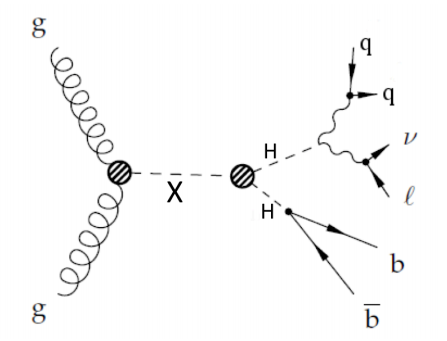
\includegraphics[scale=0.65]{figures/res_prod}
\caption[Schematic diagram of ${HH\rightarrow b\bar{b}WW^{*}\rightarrow b\bar{b}l\nu qq}$]{Schematic diagram of resonant Higgs boson pair production with the subsequent Higgs and W boson
decays.}
\label{fig:res}
\end{center}
\end{figure}

\indent This analysis sets limits on both SM Higgs boson pair production and on resonant production. Both production methods are discussed in detail in chapter \ref{chap:dihiggs}. Figure ~\ref{fig:res} shows a Feynman diagram of resonant production of the Higgs boson pairs with the subsequent decays ${H\rightarrow WW^{*}}$ and ${H\rightarrow b\overline{b}}$.
